%% Article SC-Reborn pour International Journal of Production Economics
%% ENGLISH VERSION OF THE MAIN MANUSCRIPT (the French sources stay in manuscrit/).
%% MANUSCRIT PRINCIPAL (Elsevier CAS, une colonne).
%% Le matériel supplémentaire est compilé séparément par supplement.tex,
%% avec les mêmes figures, la même bibliographie et les mêmes réglages (commun.tex).

\documentclass[a4paper,fleqn]{cas-sc}

\usepackage[T1]{fontenc}
\usepackage[english]{babel}
\usepackage[authoryear,longnamesfirst]{natbib}
\usepackage{amsmath,amssymb}
\usepackage{graphicx}
\usepackage{capt-of} % figures insérées dans le texte, à l'endroit où elles sont citées
\usepackage{tabularx}
\usepackage{enumitem}
\usepackage{tikz}
\usetikzlibrary{arrows.meta,positioning,fit,backgrounds,calc,patterns}
% Réglages communs au manuscrit et au matériel supplémentaire : couleurs, colonnes, champs à compléter.
% Couleurs des figures (politiques de gestion et paliers du réseau bayésien)
\definecolor{polnone}{HTML}{5C5B56}
\definecolor{poltard}{HTML}{EDA100}
\definecolor{polprud}{HTML}{EB6834}
\definecolor{polreac}{HTML}{2A78D6}
% Couleurs des politiques dans l'application Isomorph-Reborn
\definecolor{appnone}{HTML}{9CA3AF}
\definecolor{appprud}{HTML}{2563EB}
\definecolor{appreac}{HTML}{DC2626}
\definecolor{apptard}{HTML}{16A34A}
\definecolor{palctx}{HTML}{8A8984}
\definecolor{palpol}{HTML}{2A78D6}
\definecolor{palrep}{HTML}{EDA100}
\definecolor{palmec}{HTML}{1BAF7A}
\definecolor{palres}{HTML}{EB6834}
\usepackage{pgfplots}
\pgfplotsset{compat=1.17}
\newcolumntype{L}{>{\raggedright\arraybackslash}X}
\newcolumntype{P}[1]{>{\raggedright\arraybackslash}p{#1}}
% Champs restant à compléter avant la soumission (en bleu)
\newcommand{\acompleter}[1]{\textcolor{blue}{#1}}

% Renvois du manuscrit vers le matériel supplémentaire (numérotation S1, S2, ... fixée dans supplement.tex)
\newcommand{\voirSM}[1]{voir le matériel supplémentaire, section~#1}


% Mettre \anonymetrue pour la version soumise en double aveugle (masque auteurs, affiliations, CRediT et financement).
\newif\ifanonyme
\anonymetrue

% Title, highlights and keywords (brought back from the working document).
% The abstract is written directly in the master file: the class copies it
% verbatim to a file and does not accept a macro.
\newcommand{\ArticleTitle}{Digital twin and causal Bayesian control of supply chain resilience}
\newcommand{\ArticleHighlights}{\item Simulated crises link disruption, decision, and service level
\item Counterfactual replay isolates the effect of the managerial reaction
\item A seven-parameter curve turns service level into six resilience indicators
\item A causal Bayesian network diagnoses and predicts resilience
\item Reacting early shortens the crisis and makes each lever engaged pay off}
\newcommand{\ArticleKeywords}{supply chain resilience \sep disruption management \sep Bayesian networks \sep causal inference \sep simulation \sep resilience curve \sep decision support}


\begin{document}
\let\WriteBookmarks\relax
\def\floatpagepagefraction{1}
\def\textpagefraction{.001}

\shorttitle{Logistics network resilience: simulate, measure, learn}
\ifanonyme\shortauthors{Anonymized authors}\else\shortauthors{N. Rahiel et al.}\fi

\title [mode = title]{\ArticleTitle}

\ifanonyme
\author[1]{\acompleter{Authors anonymized for review}}
\affiliation[1]{organization={\acompleter{Anonymized}},
            country={France}}
\else
\author[1]{Naïma Rahiel}
\author[1]{Sid-Ali Addouche}
\cormark[1]
\author[1]{El Mouloudi Dafaoui}
\author[1]{Abderrahman El Mhamedi}
\author[2,3]{Saïd Amari}
\author[4]{Agnès Letouzey}
\author[4]{Xavier Desforges}
\author[4]{Kamal Medjaher}
\affiliation[1]{organization={Laboratoire QUARTZ, IUT de Montreuil, Université Paris 8},
            city={Montreuil},
            country={France}}
\affiliation[2]{organization={LURPA, ENS Paris-Saclay},
            city={Gif-sur-Yvette},
            country={France}}
\affiliation[3]{organization={LIPN, Université Sorbonne Paris Nord},
            city={Villetaneuse},
            country={France}}
\affiliation[4]{organization={LGP, Université de Toulouse, UTTOP},
            city={Tarbes},
            country={France}}
\cortext[1]{Corresponding author}
\fi

\begin{abstract}
Supply chain resilience depends as much on the reaction of operations managers as on the disruption itself, yet no database links a disruption, the decisions taken, and the resulting evolution of the service level. This article proposes a three-step approach to fill this gap. A multi-echelon logistics network is first subjected to controlled disruptions of five types, to which a simulated operations manager reacts by detecting the degradation, deciding, and escalating among nine levers. Each crisis is replayed with no reaction and then under three operations manager profiles, so that differences in service level are due to management alone. Each trajectory is then summarized by a composite hyperbolic resilience curve, from which six indicators are derived. Finally, a causal Bayesian network, whose structure follows the temporal order of a crisis and in which the management policy is an intervention, is used for prognosis, diagnosis, and recommendation. Over 2,000 crises simulated on the network of an open digital twin, the reaction shortens the crisis more than it reduces its depth. The most reactive policy avoids 73\% of the lost service, against 18\% and 14\% for the prudent and delayed policies. Each of its levers preserves on average one third of a day of sales, whereas the prudent policy is economically dominated. When the disruption duration is known, the learned network recommends a lighter policy in about one crisis in seven, without notable loss of resilience.
\end{abstract}

\begin{highlights}
\ArticleHighlights
\end{highlights}

\begin{keywords}
\ArticleKeywords
\end{keywords}

\maketitle

\section{Introduction}
\label{sec:1}

A logistics disruption, whether a supplier failure, a warehouse closure, or a demand surge, often has effects that last several weeks or even months. Its cost depends on the severity of the disruption and, just as much, on how quickly and how appropriately operations managers react \citep{sheffi2005book,ivanov2019ijpr}. A robust network absorbs the disruption without degrading. When this is not possible, its resilience, that is, its ability to limit the loss and then recover, depends largely on the decisions taken during the crisis.

Mitigation and contingency strategies are well documented \citep{tomlin2006,chopra2004}. Resilience is classically represented by a loss and recovery curve \citep{bruneau2003,rahiel2026in4pl}. It remains difficult, however, to answer two questions that operations managers ask in practice. Faced with a given disruption, which reaction is most likely to reach the target resilience level? After a poor recovery, was the loss due to the disruption, the network, or the reaction? Answering them requires observations that link a disruption, the decisions taken, and the resulting evolution of the service level. Company data are confidential and incomplete, public databases describe disruptions without the decisions, and simulation studies report only a small number of cases \citep{ramzy2022,do2024}. A deeper difficulty adds to this. A real crisis is experienced only once, under a single management, and what another reaction would have produced remains unknown. Because operations managers react more strongly when the crisis is more severe, the observed effect of a decision is mixed with that of the disruption.

This work removes this difficulty through counterfactual replay: each simulated crisis is replayed identically, first with no reaction and then under several management policies, so that any difference in trajectory is due to the decision alone. Moreover, no existing database offers this property. It is this property that allows a causal model to recommend a decision, and not merely to observe that a decision and an outcome often go together. To overcome this second difficulty, the open digital twin ISOMORPH \citep{zhang2026isomorph} was taken up and extended in a platform developed for this work, named Isomorph-Reborn.

The approach consists of three sequential blocks, as shown in Fig.~\ref{fig:d1}. The first, Simulate, produces labeled crises, that is, crises whose cause (type, target, date, duration, and severity of the disruption) and the decisions taken in response are known exactly. In this block, the multi-echelon logistics network simulated by Isomorph-Reborn is subjected to controlled disruptions to which a simulated operations manager reacts. The second, Measure, summarizes each daily service level trajectory by a seven-parameter resilience curve, from which six ``network resilience'' indicators are derived. The third, Learn, builds a causal Bayesian network on the resulting dataset. This network is used for prognosis, diagnosis, and recommendation, based on the counterfactual concept developed by the 2011 Turing Award laureate Judea Pearl \citep{pearl2009}.

\begin{center}
\resizebox{0.88\textwidth}{!}{% Figure 1: three-block approach (simplified version).
% The former detailed figure remains available: figures/Fig1_approach_EN.pdf

% --- Adjustable block dimensions -----------------------------------------
\def\bw{5.0cm}   % block width
\def\bh{3.0cm}   % block height
% -------------------------------------------------------------------------

\begin{tikzpicture}[
  font=\small,
  bloc/.style={draw=#1, line width=1pt, rounded corners=4pt, fill=#1!6,
               minimum width=\bw, minimum height=\bh},
  titre/.style={font=\small\bfseries, text=#1!80!black},
  etape/.style={draw=black!25, rounded corners=2pt, fill=white,
                text width=3.6cm, align=center, minimum height=0.62cm,
                inner sep=2pt, font=\scriptsize},
  fl/.style={-{Stealth[length=2.4mm]}, line width=1.1pt, black!55},
  pt/.style={-{Stealth[length=1.6mm]}, black!35}]

  % ---- Block 1 ---------------------------------------------------------
  \node[bloc=polreac] (B1) at (0,0) {};
  \node[titre=polreac, rotate=90, anchor=north]
        at ([xshift=7pt]B1.west) {1. Simulate};
  \node[etape] (a1) at (0.40, 0.85) {Network and labeled\\disruption};
  \node[etape] (a2) at (0.40, 0.00) {Crisis replayed: no reaction\\and 3 management profiles};
  \node[etape] (a3) at (0.40,-0.85) {Service level $\mathrm{PI}(t)$ over time};
  \draw[pt] (a1) -- (a2); \draw[pt] (a2) -- (a3);

  % ---- Block 2 ---------------------------------------------------------
  \node[bloc=palmec] (B2) at (5.6,0) {};
  \node[titre=palmec, rotate=90, anchor=north]
        at ([xshift=7pt]B2.west) {2. Measure};
  \node[etape] (b1) at (5.95, 0.45) {Associated 7-parameter resilience curves};
  \node[etape] (b2) at (5.95,-0.45) {6 network resilience\\indicators};
  \draw[pt] (b1) -- (b2);

  % ---- Block 3 ---------------------------------------------------------
  \node[bloc=polprud] (B3) at (11.2,0) {};
  \node[titre=polprud, rotate=90, anchor=north]
        at ([xshift=7pt]B3.west) {3. Learn};
  \node[etape] (c1) at (11.55, 0.45) {Causal Bayesian network};
  \node[etape] (c2) at (11.55,-0.45) {Prognosis, diagnosis, and recommendation};
  \draw[pt] (c1) -- (c2);

  % ---- Sequence --------------------------------------------------------
  \draw[fl] (B1.east) -- (B2.west);
  \draw[fl] (B2.east) -- (B3.west);
\end{tikzpicture}
}
\captionof{figure}{Three-block approach: simulate crises under four policies, measure their resilience, and learn a causal Bayesian network.}\label{fig:d1}
\end{center}

Concretely, this is a parametric platform for generation, analysis, and decision support. The generator of labeled and counterfactually replayed crises applies to any multi-echelon network. It makes inventory cover a factor of study rather than an obstacle. This generator offers a characterization of resilience whose parameters read directly in logistics terms. Finally, it builds a causal model whose structure follows the temporal order of a crisis and in which the management policy is an intervention, which makes its effect on resilience identifiable.

The next section positions this work in the literature. Section~3 describes the approach and Section~4 presents its results, which are discussed in Section~5 before the conclusion. The technical developments are gathered in a supplementary material, in particular to allow genuine repeatability by anyone. Its sections, figures, and tables carry the prefix S (Section~S3, Figure~S1, Table~S1). A reference of this form therefore always points to this supplementary material.

\section{Literature review}
\label{sec:etat}

\textbf{Four research streams} relate to recommending decisions in the face of disruptions: resilience measurement, mitigation and contingency strategies, disruption simulation, and causal Bayesian networks. Their detailed review is given in Section~S2. Here we retain what positions the approach and helps the reader grasp the contributions of this work.

The first stream measures resilience from the performance trajectory. Supply chain resilience is generally defined as the ability of a supply chain to prepare for disruptions, respond to them, and recover from them \citep{tukamuhabwa2015, kamalahmadi2016}. \citet{rahiel2026in4pl} and \citet{rahiel2026these} formalized this definition mathematically from the performance trajectory, which describes the drop and then the recovery of a disrupted supply chain. This framework was applied to the hospital supply chain \citep{rahiel2025esd} and complemented by a probabilistic modeling of severe disruptions \citep{rahiel2026codit}. Several measures thus start from the performance observed over time. \citet{bruneau2003} associate the resilience loss with the area between nominal performance and degraded performance, \citet{henry2012} treat resilience as a function of time, and others derive indicators useful for decision making \citep{spiegler2012, behzadi2020}. Building on all of this, the formalization of \citet{rahiel2026in4pl} describes the whole curve by a composite function of hyperbolic tangents with seven parameters, which yields six indicators. Note, however, that the approach assumes an already observed curve. None of these works explains how to obtain comparable curves in large numbers, for varied crises and different responses.

Measuring resilience does not say how to improve it. This is the subject of work on mitigation and contingency strategies. Mitigation measures, taken before the disruption, are distinguished from contingency measures, taken once it occurs \citep{tang2006, tomlin2006}. Quantitative studies have clarified the role of each lever, with inventory acting mainly as prevention and reserve capacity as reaction \citep{lucker2019}. They have compared proactive policies with recovery policies \citep{ivanov2016tre} and quantified the costs of resilience \citep{aldrighetti2021}. In these studies, decisions are most often fixed in advance. Their triggering as the crisis unfolds, with the detection and decision delays of a real operations manager, is rarely modeled \citep{klibi2012ijpe}. Several management policies are seldom compared against the same hazard.

Simulation has become the standard way to confront these strategies with varied disruptions. It is now the common tool for studying disruption propagation, or the domino effect, notably in supply chains \citep{schmitt2012, ivanov2017}. It also serves to build design of experiments (DoE) approaches \citep{macdonald2018}, to generate plausible scenarios \citep{klibi2012ejor}, and to compare recovery strategies \citep{ramzy2022}. ISOMORPH, to our knowledge the first public digital twin of a multi-echelon logistics network, provides reference trajectories for forecasting, without decisions that react to the state of the network \citep{zhang2026isomorph}. This simulator is designed to study one network or one case. No simulator systematically replays the same hazard with no reaction and then under several management policies.

What remains is to derive decision rules from observed or simulated crises, which Bayesian networks make possible. They represent the dependencies between risks, strategies, and consequences, and allow reasoning from cause to effect as well as from effect to cause \citep{hosseiniivanov2020}. They have been used to model risk propagation \citep{garvey2015, ojha2018} and to select mitigation strategies \citep{qazi2018}. Their structure, often set by experts, can also be learned from data, and the two sources can be combined \citep{heckerman1995}. This last point is a notable advantage. For such a model to recommend a decision, the effect of that decision must be identifiable. A decision is an intervention in the sense of \citet{pearl2009}, and its consequence cannot be read from an observed correlation, since the operations manager reacts more strongly when the crisis is more severe. Company records do not allow this causal identification, because they often contain neither the label of the decision taken nor what would have happened without it \citep{do2024}.

These four streams are well established, but they have developed separately (Table~\ref{tab:synthese}). No known public database links, for a large number of crises, the disruption suffered, the decision taken, and the resulting service level trajectory.

\begin{table*}[htbp]
\caption{Literature streams, limitations for decision recommendation, and response provided by this work.}
\label{tab:synthese}
\footnotesize
\begin{tabularx}{\textwidth}{@{}P{1.9cm}P{3.3cm}LLL@{}}
\toprule
\textbf{Stream} & \textbf{Representative works} & \textbf{Contribution} & \textbf{Limitation for recommendation} & \textbf{Response of this work} \\
\midrule
Resilience measurement
  & \citealp{bruneau2003}; \citealp{henry2012}; \citealp{spiegler2012}; \citealp{behzadi2020}; \citealp{rahiel2026in4pl}
  & Performance curve, indicators, explicit function of the trajectory
  & Assumes an already observed curve
  & Measure: seven-parameter function fitted to each simulated trajectory \\
\addlinespace
Mitigation and contingency
  & \citealp{tang2006}; \citealp{tomlin2006}; \citealp{lucker2019}; \citealp{ivanov2016tre}; \citealp{aldrighetti2021}
  & Catalog of levers and their costs
  & Decisions fixed in advance; reaction delays rarely modeled
  & Simulate: operations manager who sees only the service level, three management profiles \\
\addlinespace
Disruption simulation
  & \citealp{schmitt2012}; \citealp{ivanov2017}; \citealp{macdonald2018}; \citealp{klibi2012ejor}; \citealp{ramzy2022}; \citealp{zhang2026isomorph}
  & Propagation of disruptions, scenario generation, recovery strategies
  & Single case study; no systematic counterfactuals
  & Simulate: each crisis replayed with no reaction and then under each profile \\
\addlinespace
Causal Bayesian networks
  & \citealp{garvey2015}; \citealp{ojha2018}; \citealp{qazi2018}; \citealp{hosseiniivanov2020}; \citealp{rahiel2026codit}
  & Inference in both directions, strategy selection
  & Scarce data, without decision labels or counterfactuals
  & Learn: network learned on the counterfactual dataset, with forbidden arcs \\
\bottomrule
\end{tabularx}
\end{table*}

\section{Approach: simulate, measure, learn}
\label{sec:3}

The object of study is the crisis, followed from start to finish: what caused it, what the operations managers decided, and how the service level evolved day by day. The Simulate block produces these crises, the Measure block summarizes each one by a resilience curve, and the Learn block derives a causal model from them.

\subsection{Digital twin of the Isomorph-Reborn platform}
\label{sec:3.1}

This work starts from ISOMORPH \citep{zhang2026isomorph}, an open digital twin of a distribution network located in real cities of the United States. Three sources (San Francisco, St.~Louis, and Orlando) supply a hub in Nashville. The goods then pass through Atlanta and then through Chicago, Charlotte, Memphis, Columbus, Richmond, Philadelphia, and Baltimore to reach a single customer in New York. The network thus has thirteen cities connected by sixteen links. It is simulated with a daily time step and an (s, S) replenishment policy. ISOMORPH was designed for forecasting and is not suited as such to the study of resilience. Its disruptions are not labeled, no decision is made during a crisis, and no resilience indicator is computed.

A first attempt, which directly grafted an operations manager and disruptions onto ISOMORPH, ran into the buffer stocks. They absorbed most of the disruptions and about half of the scenarios showed no degradation. The Isomorph-Reborn platform, developed for this work, therefore extends ISOMORPH by distinguishing two nested representations of the same network. The first, called the flow representation, is an instantaneous capacitated flow model, in which any drop in the service level is explained by a loss of capacity, an increase in demand, or an identified decision. The second, called the temporal representation, adds transport and production lead times and an (s, S) inventory policy at each storage site. This makes absorption by inventory a factor that can be set at will. Isomorph-Reborn also accepts any multi-echelon network. Table~\ref{tab:isomorph} summarizes what distinguishes it from ISOMORPH.

\begin{table*}[htbp]
\caption{Positioning of the Isomorph-Reborn platform relative to the ISOMORPH digital twin.}
\label{tab:isomorph}
\footnotesize
\begin{tabularx}{\textwidth}{@{}P{2.3cm}P{3cm}L@{}}
\toprule
\textbf{Dimension} & \textbf{ISOMORPH} & \textbf{Isomorph-Reborn} \\
\toprule
Network & 13 nodes, single destination, daily time step & Any multi-echelon network; parametric network with partial redundancy and ISOMORPH network as references \\
\midrule
Dynamics & Inventory managed with (s, S) & Two nested representations: instantaneous capacitated flow, or transport and production lead times with (s, S) inventory and adjustable cover \\
\midrule
Disruptions & Random, unlabeled & Five controlled types: target, date, duration, and severity known \\
\midrule
Decisions & Parameters set before the simulation & Simulated operations manager reacting during the crisis \\
\midrule
Experimentation & Independent draws & Same crisis replayed under several management policies \\
\bottomrule
\end{tabularx}
\end{table*}

\subsection{Simulation of crisis scenarios}
\label{sec:3.2}

\paragraph{Network and service level.} The network is a directed acyclic graph that connects typed sites (suppliers, factories, hubs, warehouses, carriers) to a single final customer. The sites form two groups, production and storage. A disruption or a lever targets a site of one of these groups. The shipping capacity of a storage site is carried by its outgoing links. The effectiveness of a lever therefore depends on where the binding constraint lies in the topology as much as on its nominal magnitude. Two networks can react very differently to the same disruption and the same decision. The generator makes it possible to isolate this effect by replaying the same crises on several networks. Two networks serve as references here: a parametric network with partial redundancy (three factories, nine warehouses) and the ISOMORPH network (thirteen cities, sixteen links), whose nominal values are given in Section~S3.1.

Each day, the network can deliver a volume $F(t)$. In the flow representation, this is the maximum quantity it can route with its capacities of the day. In the temporal representation, it is what the movement of material and the inventories actually allow to be delivered. This volume serves critical items first, which account for 15 to 45\% of demand depending on the scenario. Network performance is measured by its daily service level $\mathrm{PI}(t)$, the share of customer demand actually served, in which critical items count triple:

\begin{equation}
\mathrm{PI}(t) = \frac{S_r(t) + 3\,S_c(t)}{D_r(t) + 3\,D_c(t)}, \quad S_c(t) = \min\big(F(t), D_c(t)\big), \quad S_r(t) = \min\big(F(t) - S_c(t), D_r(t)\big)
\label{eq:1}
\end{equation}

$D_{c}(t)$ and $D_{r}(t)$ denote the demands for critical and ordinary items, and $S_{c}(t)$ and $S_{r}(t)$ the quantities served. The service level equals 1 when all demand is met, and demand not served on a given day is not carried over to the next day. In the temporal representation, the levels s and S of each site are expressed in days of cover of its nominal throughput \citep{scarf1960, little1961}. The network runs for 60 days without disruption before any observation (\voirSM{S3.2}).

\paragraph{Disruptions.} Each scenario undergoes a single disruption, of one of the five types in Table~\ref{tab:d3}, which correspond to distinct failure mechanisms. Its target, start date, duration, and severity $s \in [0,1]$ are known exactly, so that the origin of each observed degradation is certain.\\

\begin{table*}[htbp]
\caption{Disruption types and mechanisms represented.}
\label{tab:d3}
\footnotesize
\begin{tabularx}{\textwidth}{@{}P{2.4cm}LLP{1.7cm}@{}}
\toprule
\textbf{Type} & \textbf{Failure mechanism} & \textbf{Modeled effect} & \textbf{Nominal severity} \\
\toprule
Supplier failure & Localized loss of upstream capacity & Production of the affected site reduced by $s$ & 0.50 to 1.00 \\
\midrule
Link cut & Break of a supply route and disorganization of the site served & Link reduced by $s$; shipping of the site served reduced by $0.7\,s$; its backup routes by $0.3\,s$ & 0.80 to 1.00 \\
\midrule
Storage site closure & Loss of a distribution node & Shipping and supply of the site reduced by $s$ & 0.80 to 1.00 \\
\midrule
Demand surge & Saturation without physical damage & Demand multiplied by $1 + 2s$ & 0.50 to 1.00 \\
\midrule
Congestion & Diffuse degradation of the whole network & Transport and shipping capacities reduced by $s$ & 0.50 to 1.00 \\
\bottomrule
\end{tabularx}
\end{table*}

The reference demand of a scenario is calibrated on the volume still deliverable during the incident, through a strain rate $u$ drawn between 0.85 and 1.15. This calibration also ensures that no degradation appears before the disruption: any observed trough comes from the crisis (\voirSM{S3.3}).

\paragraph{Simulated operations manager.} The simulated operations manager does not seek the optimal decision. It reproduces the way organizations react. It sees the crisis only through the service level averaged over a few days, so as not to be alarmed by a mere fluctuation. It declares an anomaly when this smoothed level falls below a critical threshold. Beyond this (configurable) threshold, that is, when the service level falls lower, a crisis is judged likely and the resilience of the network is mobilized. Once the anomaly is declared, the operations manager takes an analysis delay before engaging a first lever. As long as the service level then remains insufficient, it engages an additional lever at regular intervals, following its order of preference. A crisis can thus worsen through late perception, decision inertia, or overly slow escalation. The nine available levers fall into four families and come from the study of contingency strategies by \citet{sheffi2005book,ivanov2019ijpr,tomlin2006,chopra2004}. These families are ``reroute flows'', ``add capacity'', ``draw on inventory'', and ``act on the demand served''. Their nominal effects and the specific operation of the inventory levers in the temporal representation are detailed in Section~S3.4.\\

Three operations manager profiles reflect contrasting management cultures (Table~\ref{tab:d5}). The \textbf{reactive} profile detects early, decides quickly, and starts by rerouting flows. The \textbf{prudent} profile filters signals more, draws on inventory first, and escalates methodically. The \textbf{delayed} profile lets the service level degrade markedly before acting, then starts by restricting the demand served.

\begin{table*}[htbp]
\caption{Operations manager profiles (nominal values).}
\label{tab:d5}
\footnotesize
\begin{tabularx}{\textwidth}{@{}p{5cm}LLL@{}}
\toprule
\textbf{Characteristic} & \textbf{Reactive} & \textbf{Prudent} & \textbf{Delayed} \\
\toprule
Critical threshold (smoothed service level) & 0.97 & 0.92 & 0.85 \\
\midrule
Smoothing period & 1 day & 4 days & 6 days \\
\midrule
Decision delay & 1 day & 3 days & 6 days \\
\midrule
Reassessment interval & 2 days & 5 days & 8 days \\
\midrule
First levers tried & Rerouting, spot carrier & Safety stock release, inventory pre-positioning & Critical order prioritization, demand postponement \\
\bottomrule
\end{tabularx}
\end{table*}

\paragraph{Counterfactual replay.} Each crisis is played four times, with no reaction at all and then under each of the three profiles. Each of these four options is called a management policy. The four versions share the same network, the same disruption, the same demand fluctuations and, in the temporal representation, the same initial inventory state. A difference in trajectory can therefore only come from the policy. The no-reaction version shows what the crisis would have been without remediation (Fig.~\ref{fig:d3}). The policy is thus an intervention in the sense of \citet{pearl2009}, assigned independently of the situation, whereas the levers actually engaged depend on what the operations manager perceives.

\begin{center}
% Figure: crisis S0366 played under the four policies (data: ip_timeseries.csv, batch A)
% Colors identical to those of the Isomorph-Reborn application.
\begin{tikzpicture}
\begin{axis}[
  width=0.93\textwidth, height=5.6cm,
  xmin=-3, xmax=25, ymin=0.80, ymax=1.02,
  xlabel={Days since disruption onset}, ylabel={Service level $\mathrm{PI}(t)$},
  xtick={-3,0,4,7,11,14,18,21,25}, ytick={0.80,0.85,0.90,0.95,1.00},
  yticklabel style={/pgf/number format/.cd,fixed,fixed zerofill,precision=2,use period},
  tick label style={font=\scriptsize}, label style={font=\small},
  grid=major, grid style={black!8},
  legend style={font=\scriptsize, draw=none, fill=none, at={(0.5,1.02)}, anchor=south, legend columns=4, /tikz/every even column/.append style={column sep=1em}},
  every axis plot/.append style={line width=1.2pt, smooth, tension=0.6}]
  \fill[black!5] (axis cs:0,0.80) rectangle (axis cs:21,1.02);
  \draw[appreac!70, densely dashed, line width=0.6pt] (axis cs:0,0.80) -- (axis cs:0,1.02);
  \node[font=\scriptsize, text=black!60, anchor=north] at (axis cs:10.5,1.018) {Atlanta closure (21 days, severity 0.95)};
  \addplot[appnone] table[x=jour,y=none] {figures/data/fig4_S0366.dat};
  \addlegendentry{No decision}
  \addplot[appprud] table[x=jour,y=prudent] {figures/data/fig4_S0366.dat};
  \addlegendentry{Prudent}
  \addplot[appreac] table[x=jour,y=reactif] {figures/data/fig4_S0366.dat};
  \addlegendentry{Reactive}
  \addplot[apptard] table[x=jour,y=tardif] {figures/data/fig4_S0366.dat};
  \addlegendentry{Delayed}
  % detection days
  \addplot[only marks, mark=triangle*, mark size=3pt, appreac, forget plot] coordinates {(0,0.8838)};
  \addplot[only marks, mark=triangle*, mark size=3pt, appprud, forget plot] coordinates {(1,0.8468)};
  \addplot[only marks, mark=triangle*, mark size=3pt, apptard, forget plot] coordinates {(3,0.8466)};
  \node[font=\scriptsize, anchor=south east, text=black!65, fill=white, fill opacity=0.85, text opacity=1, inner sep=1.5pt] at (axis cs:24.7,0.805) {$\blacktriangle$: detection day of each profile};
\end{axis}
\end{tikzpicture}

\captionof{figure}{The same crisis played under the four policies: closure of the Atlanta warehouse for 21 days.}\label{fig:d3}
\end{center}

\paragraph{Design of experiments.} For each scenario, the network characteristics, the severity and duration of the disruption, and the strain are drawn independently from a uniform distribution over their ranges. The type and target are drawn in the same way among the possible options, with one exception: a link cut targets the main link of a site with a probability of 0.85. In the absence of field data on crisis frequency, the uniform distribution gives the same weight to all plausible values. The dataset therefore describes the scenario space and not the actual frequency of crises. Each crisis is followed over 60 days, and the generation, initialized by a seed, is reproduced identically. A global strain level, from 0 to 100, sets in a single step the intensity and duration of the disruptions, the network strain, the effectiveness of the levers, and the responsiveness of the operations managers. Level 50 corresponds to the nominal values given here (\voirSM{S3.5}).

\subsection{Computation of resilience curves and indicators}
\label{sec:3.3}

A daily trajectory is too long and too noisy to be compared as such from one crisis to another. We use here the parametric hyperbolic curve (seven parameters) and the six indicators of \citet{rahiel2026in4pl}, applying them to a large number of simulated crises. The modeled service level $p(x)$, where $x$ is the time elapsed since the onset of the disruption, chains a downward transition for the drop and an upward transition for the recovery:

\begin{equation}
p(x) = k + \frac{q}{2} - \frac{h}{2}\tanh\left(\frac{\alpha\,(x - g)}{2}\right) + \frac{h + q}{2}\tanh\left(\frac{\beta\,(x - g - d)}{2}\right)
\label{eq:5}
\end{equation}

Before the crisis (e.g., fitted curve (orange) in Fig.~\ref{fig:d4}), $p(x)$ equals $k$. At the core of the crisis, it falls to the plateau $k - h$, then settles at $k + q$ after the recovery. Four parameters describe the shape of the episode: the delay $g$ of the drop, during which the network absorbs the disruption, the duration $d$ of the degraded plateau, and the steepnesses $\alpha$ and $\beta$ of the drop and the recovery. Their detailed interpretation, as well as the constraints that guarantee an interpretable shape, are given in Section~S4.1.

Each trajectory is aligned on the onset of the disruption, so that the days preceding the crisis directly give the nominal level. The seven parameters are estimated by minimizing a robust criterion, which penalizes large deviations less heavily than least squares (\voirSM{S4.1}). \\

In a logistics crisis, recovery is rarely smooth. The successive engagement of levers causes rebounds and jolts that a curve with a single drop cannot reproduce. The robust criterion limits their influence in order to focus on the depth and width of the trough, which carry most of the information on resilience. Because this criterion is not convex, the estimation starts from several initial points taken from the observed trajectory and keeps the best solution (Fig.~\ref{fig:d4}).

\begin{center}
% Figure: observed trajectory and fitted curve, crisis S0366 with no reaction
% (data: ip_timeseries.csv and parameters from resilience_ip.csv, batch A)
\begin{tikzpicture}
\begin{axis}[
  width=0.93\textwidth, height=7cm,
  xmin=-10, xmax=24, ymin=0.80, ymax=1.03,
 xlabel={Days since disruption onset}, ylabel={Service level $\mathrm{PI}(t)$},
  xtick={-10,-5,0,5,10,15,20}, ytick={0.80,0.85,0.90,0.95,1.00},
  yticklabel style={/pgf/number format/.cd,fixed,fixed zerofill,precision=2,use period},
  tick label style={font=\scriptsize}, label style={font=\small},
  grid=major, grid style={black!8},
  legend style={font=\scriptsize, draw=none, fill=none, at={(0.5,1.02)}, anchor=south, legend columns=2, /tikz/every even column/.append style={column sep=1.2em}}]
  \addplot[polreac, line width=0.9pt, smooth, tension=0.15, mark=o, mark size=1.4pt, mark options={fill=white}] table[x=jour,y=none] {figures/data/fig4_S0366.dat};
  \addlegendentry{Observed trajectory $\mathrm{PI}(t)$}
  \addplot[polprud, line width=1.6pt] table[x=jour,y=p] {figures/data/fig5_S0366_ajuste.dat};
  \addlegendentry{Fitted curve $p(x)$, $R^2 = 0.97$}
  % levels k and k - h
  \draw[black!45, dashed] (axis cs:-10,0.9984) -- (axis cs:24,0.9984);
  \draw[black!45, dashed] (axis cs:-10,0.8538) -- (axis cs:24,0.8538);
  \node[font=\scriptsize, anchor=south west] at (axis cs:-9.5,0.9984) {$k = 0.998$};
  \node[font=\scriptsize, anchor=north west] at (axis cs:-9.5,0.8538) {$k - h = 0.854$};
  % depth h
  \draw[{Stealth[length=1.6mm]}-{Stealth[length=1.6mm]}, black!70] (axis cs:-5,0.9984) -- node[font=\scriptsize, left, fill=white, inner sep=1pt]{$h = 0.145$} (axis cs:-5,0.8538);
  % plateau duration d
  \draw[{Stealth[length=1.6mm]}-{Stealth[length=1.6mm]}, black!70] (axis cs:0,0.82) -- node[font=\scriptsize, fill=white, inner sep=1pt]{$d = 20.2$ days} (axis cs:20.24,0.82);
  \draw[black!40, densely dotted] (axis cs:0,0.80) -- (axis cs:0,0.9984);
  \draw[black!40, densely dotted] (axis cs:20.24,0.80) -- (axis cs:20.24,0.9984);
  \node[font=\scriptsize, anchor=center, align=left, text=black!75, fill=white, fill opacity=0.85, text opacity=1, inner sep=2pt] at (axis cs:10,0.94) {$g = 0$: drop from the first day\\$\alpha = 19.7$, $\beta = 96.3$: abrupt transitions\\$q \approx 0$: return to the initial level\\IPC $= 1.47$};
\end{axis}
\end{tikzpicture}

\captionof{figure}{Observed trajectory and fitted curve for the crisis of Figure~\ref{fig:d3}, with no reaction, showing how the parameters are read.}\label{fig:d4}
\end{center}

The fitted parameters give six indicators by direct computation: the cumulative loss index (IPC), the dynamic recovery coefficient (CRD), the weighted recovery time (TRP), the adaptive robustness score (SRA), the relative resilience efficiency (ERR), and the recovery potential (PR). The most used here, IPC, measures the area between the nominal level and the curve:

\begin{equation}
\mathrm{IPC} = \frac{h}{\alpha}\ln 2 + \frac{h\,d}{2} - \frac{h + q}{\beta}\ln 2
\label{eq:7}
\end{equation}

The definitions and formulas of the six indicators, as well as the estimation criterion, are given in Sections~S4.1 and S4.2. Only three of them enter the Bayesian network and the results of Section~\ref{sec:4.3}: IPC, TRP, and CRD. SRA is redundant with the parameters from which it is computed. ERR varies too little from one crisis to another to be informative. The favorable direction of PR depends on the depth of the drop (\voirSM{S5}).

The curve describes resilience in the strict sense, that is, an actual drop followed by a recovery. A crisis absorbed without degradation falls under robustness, and small, rapid variations around the nominal level fall under stability. A drop from which the network does not recover falls under failure, which calls for a reconfiguration. When $h$ tends to zero, CRD and SRA, which are normalized by $h$, become unstable. This signals an absorbed crisis, and therefore a case of robustness (\voirSM{S4.3}).

\subsection{Causal Bayesian learning}
\label{sec:3.4}

Each version of a crisis provides one observation. The variables are arranged according to the causes that a diagnosis must be able to distinguish and according to the temporal order of the crisis, which imposes tiers that no causal relation can go back up (Table~\ref{tab:d9}). The target position flags in particular the bottlenecks, that is, sites or links whose loss would cut the customer off from all its sources. Continuous variables are divided into three equal-frequency classes, whose thresholds are computed on the learning sample. The prognosis targets IPC, which closely tracks the lost service and whose direction is unambiguous.

\begin{table*}[htbp]
\caption{Variables of the learning dataset, tiers of the causal structure, and associated diagnostic question.}
\label{tab:d9}
\footnotesize
\begin{tabularx}{\textwidth}{@{}P{2.4cm}LP{2.3cm}L@{}}
\toprule
\textbf{Tier} & \textbf{Variables} & \textbf{Causal status} & \textbf{Diagnostic question} \\
\toprule
1a. Context & Target position (bottleneck, redundant site, whole network), share of critical items, type, severity, duration & Exogenous & Did the disruption hit a point with no alternative? Could it be overcome? \\
\midrule
1b. Policy & No reaction, Reactive, Prudent, Delayed & Intervention & Was the policy appropriate? \\
\midrule
2. Response & Detection delay, reaction delay, number of levers, families engaged & Mediator & Was the reaction late or poorly targeted? \\
\midrule
3. Mechanism & Parameters $h$, $d$, $\alpha$, $\beta$ & Mediator & How did the crisis unfold? \\
\midrule
4. Resilience & IPC (prognosis target), TRP, CRD & Effect & What resilience level was reached? \\
\bottomrule
\end{tabularx}
\end{table*}

Because it is assigned independently of the crisis and compared on identical crises, the policy has an effect on resilience that is identified without adjustment. The levers actually engaged, by contrast, depend on what the operations manager perceived and act as mediators. The structure is learned by greedy hill-climbing with the BIC score \citep{schwarz1978}, with the tier order imposed as forbidden arcs \citep{heckerman1995}. Inference is exact \citep{koller2009}. Learning was carried out with the BayesArtist tool \citep{bayesartist}. Any software that accepts forbidden arcs can reproduce it (\voirSM{S5}).

For a given context and policy, the learned network gives the distribution of expected resilience (prognosis) and traces a degraded resilience back to its probable causes (diagnosis). To recommend, each policy is evaluated by its probability of reaching a set resilience target. Among the policies for which this probability exceeds a threshold $\theta$ chosen by the decision maker, the least interventionist one is retained, the order being that of the mean number of levers engaged (no reaction, delayed, prudent, reactive). The policy is a root variable, assigned according to a uniform distribution. Backward inference, from the target to the policy, therefore ranks the policies exactly as the prognosis does. A single query per context is enough to draw up a recommendation map.

The results of the Bayesian network shown come from 2,000 scenarios split into 1,600 for learning and 400 for testing. Since each test crisis was played under all policies, one can check directly whether the recommended policy reached the target. The prognosis is assessed on the test crises with two standard measures. Accuracy is the share of crises whose most probable loss class according to the network is the observed class. The Brier score \citep{brier1950} assesses the probabilities themselves, on which the recommendation relies. It sums, over the three classes, the squared difference between the predicted probability and the observed outcome (1 for the observed class, 0 for the others), then averages it over the crises. It equals 0 for a perfect forecast and 0.667 for a forecast that assigns 1/3 to each class. The lower it is, the better the prognosis.

\section{Results}
\label{sec:4}

% \subsection{Generated dataset}
\label{sec:4.1}

The main dataset was generated with Isomorph-Reborn using the ISOMORPH network at a strain level of 75, in the flow representation (hence without inventory effects). Severity ranges from 0.68 to 1, disruption duration from 8 to 24 days, and the strain rate from 1.08 to 1.42. The critical thresholds of the profiles were raised to 0.98, 0.95, and 0.92. With a median minimum service level close to 0.87, the nominal thresholds left the prudent and delayed profiles almost always inactive. The ranking of the profiles, the sole object of the comparison, remains the same.

The dataset used contains the 2,000 scenarios, that is, 8,000 crisis versions, split roughly equally among the five disruption types. The curve fit is satisfactory, with a median coefficient of determination of 0.88. The cumulative loss IPC tracks the service actually lost very closely (correlation of 0.97). This is why it serves as the main indicator in what follows (\voirSM{S6.1}).

\subsection{Effect of management policies}
\label{sec:4.2}

Table~\ref{tab:d12} compares the four policies over the 2,000 crises. The reactive profile clearly comes out ahead. It reduces the cumulative loss by a median 82\% relative to no reaction, against 17\% for the prudent profile and 0\% for the delayed profile, which does not act in half of the crises. All three differences are significant (paired Wilcoxon signed-rank test, $p < 10^{-150}$). Since levers have no cost in the model, acting early never has a drawback. This advantage stems in part from the very construction of the model.


\begin{table*}[htbp]
\caption{Reaction and resilience by management policy (2,000 crises).}
\label{tab:d12}
\footnotesize
\begin{tabularx}{\textwidth}{@{}LP{2.3cm}P{2.3cm}P{2.3cm}P{2.3cm}@{}}
\toprule
\textbf{Indicator} & \textbf{No reaction} & \textbf{Reactive} & \textbf{Prudent} & \textbf{Delayed} \\
\toprule
Versions with at least one lever engaged & not applicable & 98\% & 88\% & 56\% \\
\midrule
Mean number of levers engaged & 0 & 2.8 & 2.0 & 0.7 \\
\midrule
Detection, days after onset (median) & not applicable & 0 & 1 & 3 \\
\midrule
Minimum service level (median) & 0.87 & 0.89 & 0.88 & 0.87 \\
\midrule
Days before return to normal (median) & 14 & 4 & 11 & 13 \\
\midrule
IPC, median [quartiles] & 0.67 [0.43; 1.02] & 0.11 [0.07; 0.18] & 0.51 [0.36; 0.69] & 0.58 [0.43; 0.74] \\
\midrule
Share of lost service avoided & reference & 73\% & 18\% & 14\% \\
\bottomrule
\end{tabularx}
\end{table*}

Reacting shortens the crisis without reducing its depth. The minimum service level is almost the same under all policies, but the return to normal occurs on the fourth day under the reactive profile, against the fourteenth day with no reaction (Fig.~\ref{fig:d5}). Under the reactive profile, the cumulative loss no longer depends on the disruption duration (Spearman rank correlation of 0.01), whereas it clearly does with no reaction (0.48). Severity, by contrast, carries little weight (0.08); within this range, it is the persistence of the disruption that makes the crisis.

\begin{center}
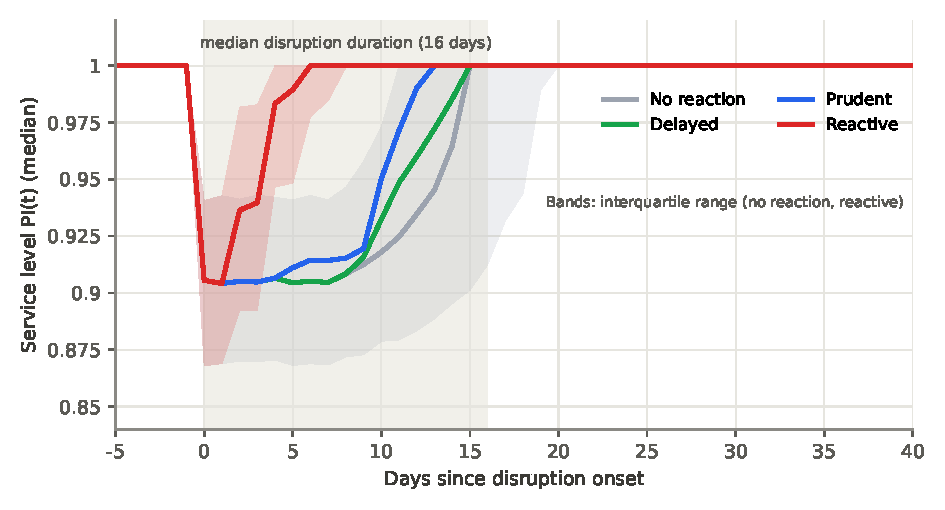
\includegraphics[width=0.5\textwidth]{figures/Fig5_median_trajectory_EN.pdf}
\captionof{figure}{Median service level trajectory by management policy (2,000 crises aligned on disruption onset).}\label{fig:d5}
\end{center}

The effectiveness of a policy varies with the disruption type. The prudent profile, for example, makes no difference to a supplier failure but reduces the loss from a congestion by 41\% (\voirSM{S6.2}). Duration also matters. If the loss is split into three levels of equal size, the prudent profile reaches the same level as the reactive profile in 18\% of the crises, a share that rises to 31\% for disruptions of 12 days or less and falls to 11\% beyond 18 days. A short crisis can therefore be handled with a light response, whereas a long crisis calls for reactivity.

These proportions hold on a second network. On a control batch of 500 scenarios generated on the parametric network, the share of lost service avoided reaches 67\%, 17\%, and 13\% for the reactive, prudent, and delayed profiles. Topology nevertheless changes the effectiveness of the levers. On this network, whose backup routes are narrow, the reactive profile reduces the loss from a link cut by only 25\% and that from a closure by 53\%, against 73\% and 82\% on ISOMORPH.

\subsection{Steering with the Bayesian model}
\label{sec:4.3}

The learned network recovers the mechanism described above on its own. Its structure (Fig.~\ref{fig:d6}) has 41 arcs, none of which runs against the tier order. The cumulative loss depends directly on the policy, the depth $h$, and the duration $d$ of the plateau. This duration in turn depends on the policy, the disruption duration, and the reaction delay.

\begin{center}
\resizebox{\textwidth}{!}{% Figure: Bayesian network learned under constraints, with the marginal distribution of each variable
% (data: .bif file exported by BayesArtist; marginals obtained by exact inference without evidence)
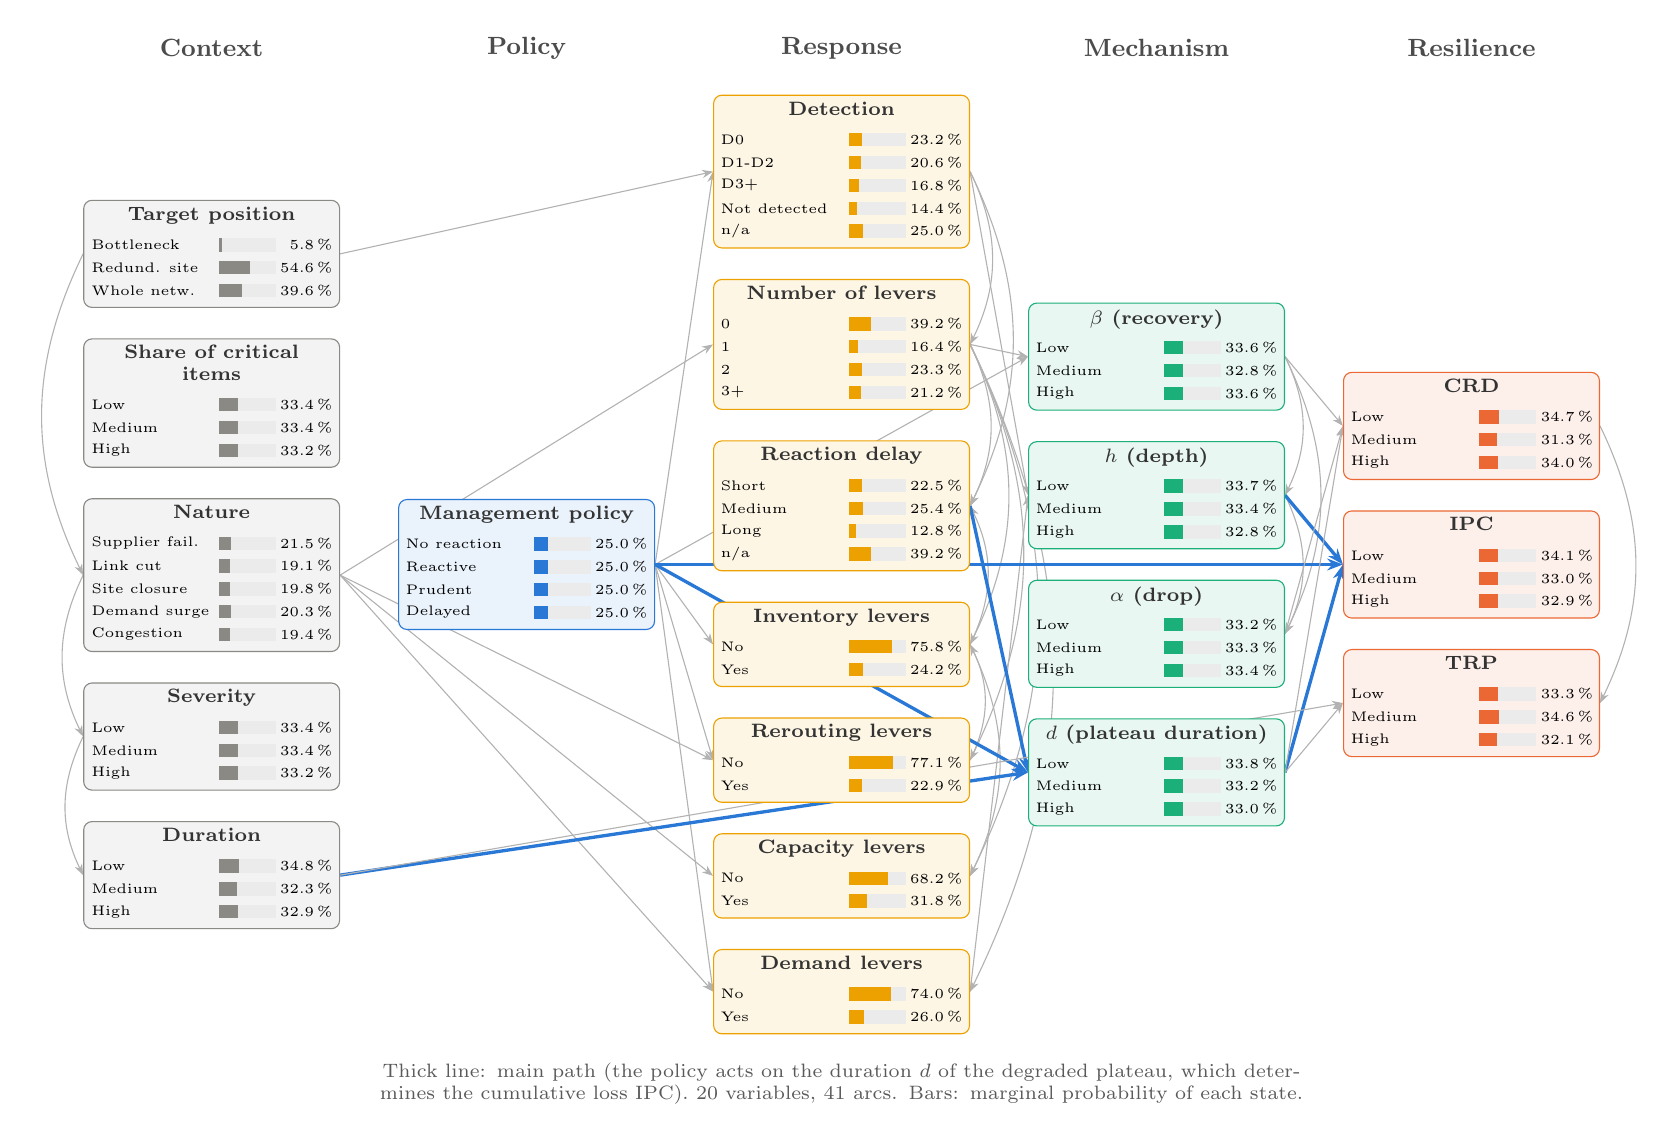
\begin{tikzpicture}[
  bx/.style={draw=#1, fill=#1!10, rounded corners=3pt, minimum width=3.25cm, inner sep=0pt},
  tt/.style={font=\scriptsize\bfseries, text=black!80, anchor=north, align=center, inner sep=1pt},
  ml/.style={font=\tiny, anchor=west, inner sep=0pt},
  pc/.style={font=\tiny, anchor=east, inner sep=0pt},
  a/.style={-{Stealth[length=1.4mm]}, black!30, thin},
  m/.style={-{Stealth[length=2mm]}, polreac, very thick}]
  \node[font=\small\bfseries, text=black!70] at (0.00,6.56) {Context};
  % cible
  \node[bx=palctx, minimum height=1.360cm] (cible) at (0.00,3.945) {};
  \node[tt] at (0.00,4.585) {Target position};
  \node[ml] at (-1.53,4.060) {Bottleneck};
  \fill[black!8] (0.095,3.975) rectangle (0.815,4.145);
  \fill[palctx] (0.095,3.975) rectangle (0.137,4.145);
  \node[pc] at (1.54,4.060) {5.8\,\%};
  \node[ml] at (-1.53,3.770) {Redund. site};
  \fill[black!8] (0.095,3.685) rectangle (0.815,3.855);
  \fill[palctx] (0.095,3.685) rectangle (0.488,3.855);
  \node[pc] at (1.54,3.770) {54.6\,\%};
  \node[ml] at (-1.53,3.480) {Whole netw.};
  \fill[black!8] (0.095,3.395) rectangle (0.815,3.565);
  \fill[palctx] (0.095,3.395) rectangle (0.380,3.565);
  \node[pc] at (1.54,3.480) {39.6\,\%};
  % partcrit
  \node[bx=palctx, minimum height=1.630cm] (partcrit) at (0.00,2.050) {};
  \node[tt] at (0.00,2.825) {Share of critical\\items};
  \node[ml] at (-1.53,2.030) {Low};
  \fill[black!8] (0.095,1.945) rectangle (0.815,2.115);
  \fill[palctx] (0.095,1.945) rectangle (0.335,2.115);
  \node[pc] at (1.54,2.030) {33.4\,\%};
  \node[ml] at (-1.53,1.740) {Medium};
  \fill[black!8] (0.095,1.655) rectangle (0.815,1.825);
  \fill[palctx] (0.095,1.655) rectangle (0.335,1.825);
  \node[pc] at (1.54,1.740) {33.4\,\%};
  \node[ml] at (-1.53,1.450) {High};
  \fill[black!8] (0.095,1.365) rectangle (0.815,1.535);
  \fill[palctx] (0.095,1.365) rectangle (0.334,1.535);
  \node[pc] at (1.54,1.450) {33.2\,\%};
  % nature
  \node[bx=palctx, minimum height=1.940cm] (nature) at (0.00,-0.135) {};
  \node[tt] at (0.00,0.795) {Nature};
  \node[ml] at (-1.53,0.270) {Supplier fail.};
  \fill[black!8] (0.095,0.185) rectangle (0.815,0.355);
  \fill[palctx] (0.095,0.185) rectangle (0.250,0.355);
  \node[pc] at (1.54,0.270) {21.5\,\%};
  \node[ml] at (-1.53,-0.020) {Link cut};
  \fill[black!8] (0.095,-0.105) rectangle (0.815,0.065);
  \fill[palctx] (0.095,-0.105) rectangle (0.233,0.065);
  \node[pc] at (1.54,-0.020) {19.1\,\%};
  \node[ml] at (-1.53,-0.310) {Site closure};
  \fill[black!8] (0.095,-0.395) rectangle (0.815,-0.225);
  \fill[palctx] (0.095,-0.395) rectangle (0.238,-0.225);
  \node[pc] at (1.54,-0.310) {19.8\,\%};
  \node[ml] at (-1.53,-0.600) {Demand surge};
  \fill[black!8] (0.095,-0.685) rectangle (0.815,-0.515);
  \fill[palctx] (0.095,-0.685) rectangle (0.241,-0.515);
  \node[pc] at (1.54,-0.600) {20.3\,\%};
  \node[ml] at (-1.53,-0.890) {Congestion};
  \fill[black!8] (0.095,-0.975) rectangle (0.815,-0.805);
  \fill[palctx] (0.095,-0.975) rectangle (0.235,-0.805);
  \node[pc] at (1.54,-0.890) {19.4\,\%};
  % severite
  \node[bx=palctx, minimum height=1.360cm] (severite) at (0.00,-2.185) {};
  \node[tt] at (0.00,-1.545) {Severity};
  \node[ml] at (-1.53,-2.070) {Low};
  \fill[black!8] (0.095,-2.155) rectangle (0.815,-1.985);
  \fill[palctx] (0.095,-2.155) rectangle (0.335,-1.985);
  \node[pc] at (1.54,-2.070) {33.4\,\%};
  \node[ml] at (-1.53,-2.360) {Medium};
  \fill[black!8] (0.095,-2.445) rectangle (0.815,-2.275);
  \fill[palctx] (0.095,-2.445) rectangle (0.335,-2.275);
  \node[pc] at (1.54,-2.360) {33.4\,\%};
  \node[ml] at (-1.53,-2.650) {High};
  \fill[black!8] (0.095,-2.735) rectangle (0.815,-2.565);
  \fill[palctx] (0.095,-2.735) rectangle (0.334,-2.565);
  \node[pc] at (1.54,-2.650) {33.2\,\%};
  % duree
  \node[bx=palctx, minimum height=1.360cm] (duree) at (0.00,-3.945) {};
  \node[tt] at (0.00,-3.305) {Duration};
  \node[ml] at (-1.53,-3.830) {Low};
  \fill[black!8] (0.095,-3.915) rectangle (0.815,-3.745);
  \fill[palctx] (0.095,-3.915) rectangle (0.346,-3.745);
  \node[pc] at (1.54,-3.830) {34.8\,\%};
  \node[ml] at (-1.53,-4.120) {Medium};
  \fill[black!8] (0.095,-4.205) rectangle (0.815,-4.035);
  \fill[palctx] (0.095,-4.205) rectangle (0.328,-4.035);
  \node[pc] at (1.54,-4.120) {32.3\,\%};
  \node[ml] at (-1.53,-4.410) {High};
  \fill[black!8] (0.095,-4.495) rectangle (0.815,-4.325);
  \fill[palctx] (0.095,-4.495) rectangle (0.332,-4.325);
  \node[pc] at (1.54,-4.410) {32.9\,\%};
  \node[font=\small\bfseries, text=black!70] at (4.00,6.56) {Policy};
  % profil
  \node[bx=palpol, minimum height=1.650cm] (profil) at (4.00,0.000) {};
  \node[tt] at (4.00,0.785) {Management policy};
  \node[ml] at (2.46,0.260) {No reaction};
  \fill[black!8] (4.095,0.175) rectangle (4.815,0.345);
  \fill[palpol] (4.095,0.175) rectangle (4.275,0.345);
  \node[pc] at (5.54,0.260) {25.0\,\%};
  \node[ml] at (2.46,-0.030) {Reactive};
  \fill[black!8] (4.095,-0.115) rectangle (4.815,0.055);
  \fill[palpol] (4.095,-0.115) rectangle (4.275,0.055);
  \node[pc] at (5.54,-0.030) {25.0\,\%};
  \node[ml] at (2.46,-0.320) {Prudent};
  \fill[black!8] (4.095,-0.405) rectangle (4.815,-0.235);
  \fill[palpol] (4.095,-0.405) rectangle (4.275,-0.235);
  \node[pc] at (5.54,-0.320) {25.0\,\%};
  \node[ml] at (2.46,-0.610) {Delayed};
  \fill[black!8] (4.095,-0.695) rectangle (4.815,-0.525);
  \fill[palpol] (4.095,-0.695) rectangle (4.275,-0.525);
  \node[pc] at (5.54,-0.610) {25.0\,\%};
  \node[font=\small\bfseries, text=black!70] at (8.00,6.56) {Response};
  % detection
  \node[bx=palrep, minimum height=1.940cm] (detection) at (8.00,4.990) {};
  \node[tt] at (8.00,5.920) {Detection};
  \node[ml] at (6.46,5.395) {D0};
  \fill[black!8] (8.095,5.310) rectangle (8.815,5.480);
  \fill[palrep] (8.095,5.310) rectangle (8.262,5.480);
  \node[pc] at (9.54,5.395) {23.2\,\%};
  \node[ml] at (6.46,5.105) {D1-D2};
  \fill[black!8] (8.095,5.020) rectangle (8.815,5.190);
  \fill[palrep] (8.095,5.020) rectangle (8.243,5.190);
  \node[pc] at (9.54,5.105) {20.6\,\%};
  \node[ml] at (6.46,4.815) {D3+};
  \fill[black!8] (8.095,4.730) rectangle (8.815,4.900);
  \fill[palrep] (8.095,4.730) rectangle (8.216,4.900);
  \node[pc] at (9.54,4.815) {16.8\,\%};
  \node[ml] at (6.46,4.525) {Not detected};
  \fill[black!8] (8.095,4.440) rectangle (8.815,4.610);
  \fill[palrep] (8.095,4.440) rectangle (8.199,4.610);
  \node[pc] at (9.54,4.525) {14.4\,\%};
  \node[ml] at (6.46,4.235) {n/a};
  \fill[black!8] (8.095,4.150) rectangle (8.815,4.320);
  \fill[palrep] (8.095,4.150) rectangle (8.275,4.320);
  \node[pc] at (9.54,4.235) {25.0\,\%};
  % nbleviers
  \node[bx=palrep, minimum height=1.650cm] (nbleviers) at (8.00,2.795) {};
  \node[tt] at (8.00,3.580) {Number of levers};
  \node[ml] at (6.46,3.055) {0};
  \fill[black!8] (8.095,2.970) rectangle (8.815,3.140);
  \fill[palrep] (8.095,2.970) rectangle (8.377,3.140);
  \node[pc] at (9.54,3.055) {39.2\,\%};
  \node[ml] at (6.46,2.765) {1};
  \fill[black!8] (8.095,2.680) rectangle (8.815,2.850);
  \fill[palrep] (8.095,2.680) rectangle (8.213,2.850);
  \node[pc] at (9.54,2.765) {16.4\,\%};
  \node[ml] at (6.46,2.475) {2};
  \fill[black!8] (8.095,2.390) rectangle (8.815,2.560);
  \fill[palrep] (8.095,2.390) rectangle (8.263,2.560);
  \node[pc] at (9.54,2.475) {23.3\,\%};
  \node[ml] at (6.46,2.185) {3+};
  \fill[black!8] (8.095,2.100) rectangle (8.815,2.270);
  \fill[palrep] (8.095,2.100) rectangle (8.248,2.270);
  \node[pc] at (9.54,2.185) {21.2\,\%};
  % lag
  \node[bx=palrep, minimum height=1.650cm] (lag) at (8.00,0.745) {};
  \node[tt] at (8.00,1.530) {Reaction delay};
  \node[ml] at (6.46,1.005) {Short};
  \fill[black!8] (8.095,0.920) rectangle (8.815,1.090);
  \fill[palrep] (8.095,0.920) rectangle (8.257,1.090);
  \node[pc] at (9.54,1.005) {22.5\,\%};
  \node[ml] at (6.46,0.715) {Medium};
  \fill[black!8] (8.095,0.630) rectangle (8.815,0.800);
  \fill[palrep] (8.095,0.630) rectangle (8.278,0.800);
  \node[pc] at (9.54,0.715) {25.4\,\%};
  \node[ml] at (6.46,0.425) {Long};
  \fill[black!8] (8.095,0.340) rectangle (8.815,0.510);
  \fill[palrep] (8.095,0.340) rectangle (8.187,0.510);
  \node[pc] at (9.54,0.425) {12.8\,\%};
  \node[ml] at (6.46,0.135) {n/a};
  \fill[black!8] (8.095,0.050) rectangle (8.815,0.220);
  \fill[palrep] (8.095,0.050) rectangle (8.377,0.220);
  \node[pc] at (9.54,0.135) {39.2\,\%};
  % fstock
  \node[bx=palrep, minimum height=1.070cm] (fstock) at (8.00,-1.015) {};
  \node[tt] at (8.00,-0.520) {Inventory levers};
  \node[ml] at (6.46,-1.045) {No};
  \fill[black!8] (8.095,-1.130) rectangle (8.815,-0.960);
  \fill[palrep] (8.095,-1.130) rectangle (8.641,-0.960);
  \node[pc] at (9.54,-1.045) {75.8\,\%};
  \node[ml] at (6.46,-1.335) {Yes};
  \fill[black!8] (8.095,-1.420) rectangle (8.815,-1.250);
  \fill[palrep] (8.095,-1.420) rectangle (8.269,-1.250);
  \node[pc] at (9.54,-1.335) {24.2\,\%};
  % freroutage
  \node[bx=palrep, minimum height=1.070cm] (freroutage) at (8.00,-2.485) {};
  \node[tt] at (8.00,-1.990) {Rerouting levers};
  \node[ml] at (6.46,-2.515) {No};
  \fill[black!8] (8.095,-2.600) rectangle (8.815,-2.430);
  \fill[palrep] (8.095,-2.600) rectangle (8.650,-2.430);
  \node[pc] at (9.54,-2.515) {77.1\,\%};
  \node[ml] at (6.46,-2.805) {Yes};
  \fill[black!8] (8.095,-2.890) rectangle (8.815,-2.720);
  \fill[palrep] (8.095,-2.890) rectangle (8.260,-2.720);
  \node[pc] at (9.54,-2.805) {22.9\,\%};
  % fcapacite
  \node[bx=palrep, minimum height=1.070cm] (fcapacite) at (8.00,-3.955) {};
  \node[tt] at (8.00,-3.460) {Capacity levers};
  \node[ml] at (6.46,-3.985) {No};
  \fill[black!8] (8.095,-4.070) rectangle (8.815,-3.900);
  \fill[palrep] (8.095,-4.070) rectangle (8.586,-3.900);
  \node[pc] at (9.54,-3.985) {68.2\,\%};
  \node[ml] at (6.46,-4.275) {Yes};
  \fill[black!8] (8.095,-4.360) rectangle (8.815,-4.190);
  \fill[palrep] (8.095,-4.360) rectangle (8.324,-4.190);
  \node[pc] at (9.54,-4.275) {31.8\,\%};
  % fdemande
  \node[bx=palrep, minimum height=1.070cm] (fdemande) at (8.00,-5.425) {};
  \node[tt] at (8.00,-4.930) {Demand levers};
  \node[ml] at (6.46,-5.455) {No};
  \fill[black!8] (8.095,-5.540) rectangle (8.815,-5.370);
  \fill[palrep] (8.095,-5.540) rectangle (8.628,-5.370);
  \node[pc] at (9.54,-5.455) {74.0\,\%};
  \node[ml] at (6.46,-5.745) {Yes};
  \fill[black!8] (8.095,-5.830) rectangle (8.815,-5.660);
  \fill[palrep] (8.095,-5.830) rectangle (8.282,-5.660);
  \node[pc] at (9.54,-5.745) {26.0\,\%};
  \node[font=\small\bfseries, text=black!70] at (12.00,6.56) {Mechanism};
  % beta
  \node[bx=palmec, minimum height=1.360cm] (beta) at (12.00,2.640) {};
  \node[tt] at (12.00,3.280) {$\beta$ (recovery)};
  \node[ml] at (10.46,2.755) {Low};
  \fill[black!8] (12.095,2.670) rectangle (12.815,2.840);
  \fill[palmec] (12.095,2.670) rectangle (12.337,2.840);
  \node[pc] at (13.54,2.755) {33.6\,\%};
  \node[ml] at (10.46,2.465) {Medium};
  \fill[black!8] (12.095,2.380) rectangle (12.815,2.550);
  \fill[palmec] (12.095,2.380) rectangle (12.331,2.550);
  \node[pc] at (13.54,2.465) {32.8\,\%};
  \node[ml] at (10.46,2.175) {High};
  \fill[black!8] (12.095,2.090) rectangle (12.815,2.260);
  \fill[palmec] (12.095,2.090) rectangle (12.337,2.260);
  \node[pc] at (13.54,2.175) {33.6\,\%};
  % h
  \node[bx=palmec, minimum height=1.360cm] (h) at (12.00,0.880) {};
  \node[tt] at (12.00,1.520) {$h$ (depth)};
  \node[ml] at (10.46,0.995) {Low};
  \fill[black!8] (12.095,0.910) rectangle (12.815,1.080);
  \fill[palmec] (12.095,0.910) rectangle (12.338,1.080);
  \node[pc] at (13.54,0.995) {33.7\,\%};
  \node[ml] at (10.46,0.705) {Medium};
  \fill[black!8] (12.095,0.620) rectangle (12.815,0.790);
  \fill[palmec] (12.095,0.620) rectangle (12.335,0.790);
  \node[pc] at (13.54,0.705) {33.4\,\%};
  \node[ml] at (10.46,0.415) {High};
  \fill[black!8] (12.095,0.330) rectangle (12.815,0.500);
  \fill[palmec] (12.095,0.330) rectangle (12.331,0.500);
  \node[pc] at (13.54,0.415) {32.8\,\%};
  % alpha
  \node[bx=palmec, minimum height=1.360cm] (alpha) at (12.00,-0.880) {};
  \node[tt] at (12.00,-0.240) {$\alpha$ (drop)};
  \node[ml] at (10.46,-0.765) {Low};
  \fill[black!8] (12.095,-0.850) rectangle (12.815,-0.680);
  \fill[palmec] (12.095,-0.850) rectangle (12.334,-0.680);
  \node[pc] at (13.54,-0.765) {33.2\,\%};
  \node[ml] at (10.46,-1.055) {Medium};
  \fill[black!8] (12.095,-1.140) rectangle (12.815,-0.970);
  \fill[palmec] (12.095,-1.140) rectangle (12.335,-0.970);
  \node[pc] at (13.54,-1.055) {33.3\,\%};
  \node[ml] at (10.46,-1.345) {High};
  \fill[black!8] (12.095,-1.430) rectangle (12.815,-1.260);
  \fill[palmec] (12.095,-1.430) rectangle (12.335,-1.260);
  \node[pc] at (13.54,-1.345) {33.4\,\%};
  % d
  \node[bx=palmec, minimum height=1.360cm] (d) at (12.00,-2.640) {};
  \node[tt] at (12.00,-2.000) {$d$ (plateau duration)};
  \node[ml] at (10.46,-2.525) {Low};
  \fill[black!8] (12.095,-2.610) rectangle (12.815,-2.440);
  \fill[palmec] (12.095,-2.610) rectangle (12.338,-2.440);
  \node[pc] at (13.54,-2.525) {33.8\,\%};
  \node[ml] at (10.46,-2.815) {Medium};
  \fill[black!8] (12.095,-2.900) rectangle (12.815,-2.730);
  \fill[palmec] (12.095,-2.900) rectangle (12.334,-2.730);
  \node[pc] at (13.54,-2.815) {33.2\,\%};
  \node[ml] at (10.46,-3.105) {High};
  \fill[black!8] (12.095,-3.190) rectangle (12.815,-3.020);
  \fill[palmec] (12.095,-3.190) rectangle (12.333,-3.020);
  \node[pc] at (13.54,-3.105) {33.0\,\%};
  \node[font=\small\bfseries, text=black!70] at (16.00,6.56) {Resilience};
  % CRD
  \node[bx=palres, minimum height=1.360cm] (CRD) at (16.00,1.760) {};
  \node[tt] at (16.00,2.400) {CRD};
  \node[ml] at (14.46,1.875) {Low};
  \fill[black!8] (16.095,1.790) rectangle (16.815,1.960);
  \fill[palres] (16.095,1.790) rectangle (16.345,1.960);
  \node[pc] at (17.55,1.875) {34.7\,\%};
  \node[ml] at (14.46,1.585) {Medium};
  \fill[black!8] (16.095,1.500) rectangle (16.815,1.670);
  \fill[palres] (16.095,1.500) rectangle (16.320,1.670);
  \node[pc] at (17.55,1.585) {31.3\,\%};
  \node[ml] at (14.46,1.295) {High};
  \fill[black!8] (16.095,1.210) rectangle (16.815,1.380);
  \fill[palres] (16.095,1.210) rectangle (16.340,1.380);
  \node[pc] at (17.55,1.295) {34.0\,\%};
  % IPC
  \node[bx=palres, minimum height=1.360cm] (IPC) at (16.00,0.000) {};
  \node[tt] at (16.00,0.640) {IPC};
  \node[ml] at (14.46,0.115) {Low};
  \fill[black!8] (16.095,0.030) rectangle (16.815,0.200);
  \fill[palres] (16.095,0.030) rectangle (16.341,0.200);
  \node[pc] at (17.55,0.115) {34.1\,\%};
  \node[ml] at (14.46,-0.175) {Medium};
  \fill[black!8] (16.095,-0.260) rectangle (16.815,-0.090);
  \fill[palres] (16.095,-0.260) rectangle (16.333,-0.090);
  \node[pc] at (17.55,-0.175) {33.0\,\%};
  \node[ml] at (14.46,-0.465) {High};
  \fill[black!8] (16.095,-0.550) rectangle (16.815,-0.380);
  \fill[palres] (16.095,-0.550) rectangle (16.332,-0.380);
  \node[pc] at (17.55,-0.465) {32.9\,\%};
  % TRP
  \node[bx=palres, minimum height=1.360cm] (TRP) at (16.00,-1.760) {};
  \node[tt] at (16.00,-1.120) {TRP};
  \node[ml] at (14.46,-1.645) {Low};
  \fill[black!8] (16.095,-1.730) rectangle (16.815,-1.560);
  \fill[palres] (16.095,-1.730) rectangle (16.335,-1.560);
  \node[pc] at (17.55,-1.645) {33.3\,\%};
  \node[ml] at (14.46,-1.935) {Medium};
  \fill[black!8] (16.095,-2.020) rectangle (16.815,-1.850);
  \fill[palres] (16.095,-2.020) rectangle (16.344,-1.850);
  \node[pc] at (17.55,-1.935) {34.6\,\%};
  \node[ml] at (14.46,-2.225) {High};
  \fill[black!8] (16.095,-2.310) rectangle (16.815,-2.140);
  \fill[palres] (16.095,-2.310) rectangle (16.326,-2.140);
  \node[pc] at (17.55,-2.225) {32.1\,\%};
  \begin{scope}[on background layer]
    \draw[a] (cible.west) to[bend right=26] (nature.west);
    \draw[a] (cible.east) -- (detection.west);
    \draw[a] (profil.east) -- (detection.west);
    \draw[a] (nature.west) to[bend right=26] (severite.west);
    \draw[a] (nature.east) -- (nbleviers.west);
    \draw[a] (detection.east) to[bend left=26] (nbleviers.east);
    \draw[a] (severite.west) to[bend right=26] (duree.west);
    \draw[a] (profil.east) -- (beta.west);
    \draw[a] (nbleviers.east) -- (beta.west);
    \draw[a] (nature.east) -- (freroutage.west);
    \draw[a] (profil.east) -- (freroutage.west);
    \draw[a] (nbleviers.east) to[bend left=26] (freroutage.east);
    \draw[a] (nature.east) -- (fdemande.west);
    \draw[a] (profil.east) -- (fdemande.west);
    \draw[a] (nbleviers.east) to[bend left=26] (fdemande.east);
    \draw[a] (beta.east) to[bend left=26] (h.east);
    \draw[a] (detection.east) -- (h.west);
    \draw[a] (fdemande.east) -- (h.west);
    \draw[a] (profil.east) -- (fstock.west);
    \draw[a] (nbleviers.east) to[bend left=26] (fstock.east);
    \draw[a] (freroutage.east) to[bend right=26] (fstock.east);
    \draw[a] (h.east) to[bend left=26] (alpha.east);
    \draw[a] (beta.east) to[bend left=26] (alpha.east);
    \draw[a] (detection.east) to[bend left=26] (lag.east);
    \draw[a] (nbleviers.east) to[bend left=26] (lag.east);
    \draw[a] (fstock.east) to[bend right=26] (lag.east);
    \draw[a] (nature.east) -- (fcapacite.west);
    \draw[a] (nbleviers.east) to[bend left=26] (fcapacite.east);
    \draw[a] (fstock.east) to[bend left=26] (fcapacite.east);
    \draw[m] (profil.east) -- (d.west);
    \draw[m] (duree.east) -- (d.west);
    \draw[m] (lag.east) -- (d.west);
    \draw[m] (profil.east) -- (IPC.west);
    \draw[m] (h.east) -- (IPC.west);
    \draw[m] (d.east) -- (IPC.west);
    \draw[a] (d.east) -- (CRD.west);
    \draw[a] (alpha.east) -- (CRD.west);
    \draw[a] (beta.east) -- (CRD.west);
    \draw[a] (duree.east) -- (TRP.west);
    \draw[a] (d.east) -- (TRP.west);
    \draw[a] (CRD.east) to[bend left=26] (TRP.east);
  \end{scope}
  \node[font=\scriptsize, text=black!65, anchor=north, text width=17cm, align=center] at (8.00,-6.21) {Thick line: main path (the policy acts on the duration $d$ of the degraded plateau, which determines the cumulative loss IPC). 20 variables, 41 arcs. Bars: marginal probability of each state.};
\end{tikzpicture}
}
\captionof{figure}{Bayesian network learned under constraints, with variables colored by tier of the temporal order of a crisis; each node gives the marginal probability of its states.}\label{fig:d6}
\end{center}

Using only the variables known at decision time, the prognosis correctly classifies 65\% of the test crises, against 60\% for a model that knows only the management policy applied (no reaction, reactive, prudent, or delayed) and 34\% for an uninformed model, which assigns each class its frequency and selects the most frequent one. The corresponding Brier scores are 0.466, 0.494, and 0.667. The learning curve is almost flat, which indicates that accuracy is limited by the information available at decision time rather than by the size of the dataset. The diagnosis is well calibrated for policy and duration. For the high-loss test crises, the posterior probabilities of the policies reproduce their observed frequencies to within 0.01.

The recommendation that can be made depends on the objective. If the aim is a low loss, only the reactive profile succeeds consistently and the rule always recommends it. If the aim is only to avoid a high loss, a trade-off appears between safety and restraint, governed by the threshold $\theta$ (Table~\ref{tab:d15}).

\begin{table*}[htbp]
\caption{Recommendation on the test crises, with the objective of a cumulative loss that is not high.}
\label{tab:d15}
\footnotesize
\begin{tabularx}{\textwidth}{@{}LLL@{}}
\toprule
\textbf{Rule} & \textbf{Objective met} & \textbf{Recommendations lighter than the reactive profile} \\
\midrule
Always the reactive profile & 99.2\% & 0\% \\
Learned network, $\theta$ = 0.9 & 99.2\% & 0\% \\
Learned network, $\theta$ = 0.8 & 97.5\% & 15\% \\
Learned network, $\theta$ = 0.7 & 86.2\% & 37\% \\
Learned network, $\theta$ = 0.6 & 69.5\% & 84\% \\
A posteriori reference: lightest successful policy & 99.2\% & 67\% \\
\bottomrule
\end{tabularx}
\end{table*}

With $\theta$ = 0.8, that is, selecting the least interventionist policy among those that meet the objective with a probability of at least 0.8, the network recommends a lighter policy in about one crisis out of seven. The objective is met in 97.5\% of cases, less than two points below the most interventionist policy. This restraint rests entirely on the forecast duration of the disruption. If this information is removed from the crisis description, the rule no longer recommends any lighter policy. Knowing the probable duration of a disruption therefore has decision value in itself. For the short closure of a redundant site, for example, the prudent profile meets the objective with a probability of 0.80 and becomes the recommendation, whereas for the long closure of a bottleneck, only the reactive profile does so (\voirSM{S6.3}).

Figure~\ref{fig:carte} extends this analysis to the seven contexts allowed by the ISOMORPH topology, by backward inference and for the objective of a low loss. The reactive profile is the most probable everywhere, and all the more so as the disruption lasts longer, its posterior probability rising from 0.51--0.58 for a short disruption to 0.72--0.79 for a long one. For a short disruption, each of the other policies keeps a probability between 0.12 and 0.18, a sign that a low loss then remains attainable without a rapid reaction.

\begin{center}
\begin{minipage}{\textwidth}\centering
% Figure: recommendation map by backward inference on the learned network, as a scatter plot.
% Posterior probability of each profile given IPC = low, for the seven contexts (nature, target position),
% one panel per disruption duration. Green: most probable policy of the context; red: other policies.
% Values identical to the former map (exact inference on the learned network, .bif file).
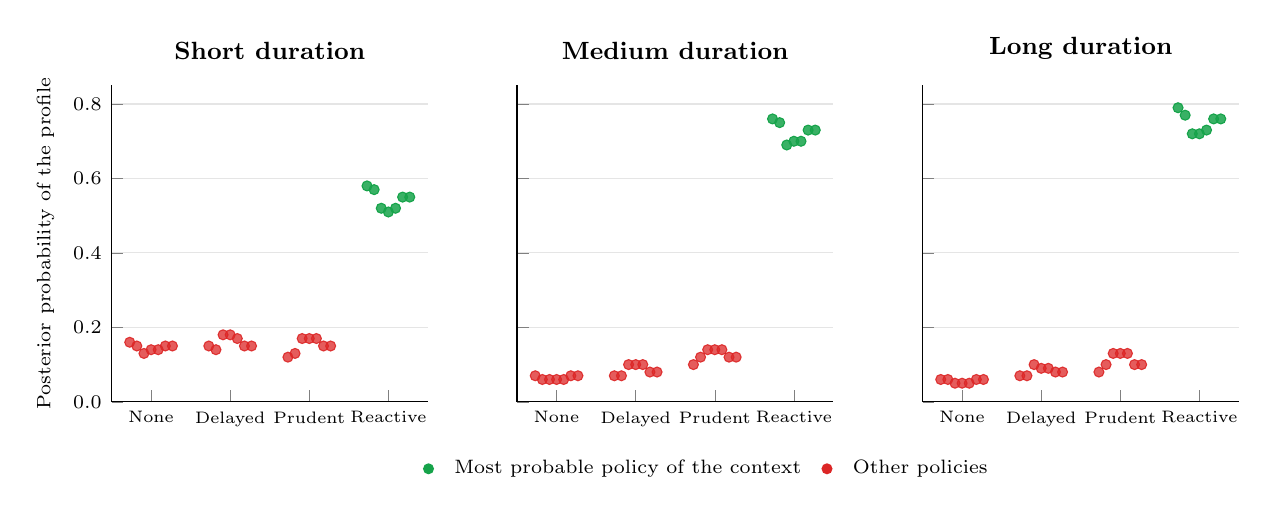
\begin{tikzpicture}
\pgfplotsset{carte/.style={width=5.6cm, height=5.6cm, xmin=0.5, xmax=4.5, ymin=0, ymax=0.85,
  xtick={1,2,3,4}, xticklabels={None,Delayed,Prudent,Reactive},
  ytick={0,0.2,0.4,0.6,0.8}, yticklabel style={/pgf/number format/.cd,fixed,fixed zerofill,precision=1,use period},
  tick label style={font=\scriptsize}, xticklabel style={font=\fontsize{6}{7}\selectfont}, label style={font=\scriptsize}, title style={font=\small\bfseries},
  ymajorgrids, grid style={gray!20}, axis lines*=left, clip=false}}
\begin{axis}[carte, title={Short duration}, at={(0.0cm,0)}, ylabel={Posterior probability of the profile}]
  \addplot[only marks, mark=*, mark size=1.8pt, appreac, fill opacity=0.75, draw opacity=0.9] coordinates {(0.73,0.16) (1.73,0.15) (2.73,0.12) (0.82,0.15) (1.82,0.14) (2.82,0.13) (0.91,0.13) (1.91,0.18) (2.91,0.17) (1.00,0.14) (2.00,0.18) (3.00,0.17) (1.09,0.14) (2.09,0.17) (3.09,0.17) (1.18,0.15) (2.18,0.15) (3.18,0.15) (1.27,0.15) (2.27,0.15) (3.27,0.15)};
  \addplot[only marks, mark=*, mark size=1.8pt, apptard, fill opacity=0.85] coordinates {(3.73,0.58) (3.82,0.57) (3.91,0.52) (4.00,0.51) (4.09,0.52) (4.18,0.55) (4.27,0.55)};
\end{axis}
\begin{axis}[carte, title={Medium duration}, at={(5.15cm,0)}, yticklabels={}]
  \addplot[only marks, mark=*, mark size=1.8pt, appreac, fill opacity=0.75, draw opacity=0.9] coordinates {(0.73,0.07) (1.73,0.07) (2.73,0.10) (0.82,0.06) (1.82,0.07) (2.82,0.12) (0.91,0.06) (1.91,0.10) (2.91,0.14) (1.00,0.06) (2.00,0.10) (3.00,0.14) (1.09,0.06) (2.09,0.10) (3.09,0.14) (1.18,0.07) (2.18,0.08) (3.18,0.12) (1.27,0.07) (2.27,0.08) (3.27,0.12)};
  \addplot[only marks, mark=*, mark size=1.8pt, apptard, fill opacity=0.85] coordinates {(3.73,0.76) (3.82,0.75) (3.91,0.69) (4.00,0.70) (4.09,0.70) (4.18,0.73) (4.27,0.73)};
\end{axis}
\begin{axis}[carte, title={Long duration}, at={(10.3cm,0)}, yticklabels={}]
  \addplot[only marks, mark=*, mark size=1.8pt, appreac, fill opacity=0.75, draw opacity=0.9] coordinates {(0.73,0.06) (1.73,0.07) (2.73,0.08) (0.82,0.06) (1.82,0.07) (2.82,0.10) (0.91,0.05) (1.91,0.10) (2.91,0.13) (1.00,0.05) (2.00,0.09) (3.00,0.13) (1.09,0.05) (2.09,0.09) (3.09,0.13) (1.18,0.06) (2.18,0.08) (3.18,0.10) (1.27,0.06) (2.27,0.08) (3.27,0.10)};
  \addplot[only marks, mark=*, mark size=1.8pt, apptard, fill opacity=0.85] coordinates {(3.73,0.79) (3.82,0.77) (3.91,0.72) (4.00,0.72) (4.09,0.73) (4.18,0.76) (4.27,0.76)};
\end{axis}
\matrix[anchor=north, font=\scriptsize, column sep=4pt] at (7.6cm,-0.5cm) {
  \fill[apptard] (0,0) circle (2pt); & \node[anchor=west]{Most probable policy of the context}; &
  \fill[appreac] (0,0) circle (2pt); & \node[anchor=west]{Other policies}; \\
};
\end{tikzpicture}

\captionof{figure}{Recommendation map: posterior probability of each profile given a low cumulative loss, for the seven contexts of disruption type and target position, by disruption duration.}\label{fig:carte}
\end{minipage}
\end{center}

% \subsection{Role of inventories}
\label{sec:4.4}

\textbf{Role of inventories — }Inventories protect against some disruptions only. The main dataset neutralizes them. To study them, we switch to the temporal representation, in which material flows with its travel and production delays and each storage site manages its inventory under an (s, S) inventory policy; 60 no-reaction crises were simulated in this representation on the ISOMORPH network for each disruption type and each inventory cover. Against distribution disruptions, inventory cover acts as a progressive robustness lever. The number of visible crises increases as cover decreases, from 11 to 43 out of 60 for a link cut. A demand surge, on the other hand, is better absorbed without inventories, because the extra demand must first be drawn from inventories sized for the nominal throughput (\voirSM{S6.4}).

\subsection{Economic analysis}
\label{sec:4.5}

The service loss is converted into lost sales by multiplying it by the reference daily demand, over the 60 days following the disruption. A no-reaction crisis thus costs 25,550 units on average, or about 1.4 days of demand. As the model does not put a cost on the levers, their cost $c$ per engagement is expressed in units of margin $m$. A policy is profitable as long as its preserved sales, multiplied by $m$, cover the cost of the levers it engages; the ratio $c/m$ beyond which it ceases to be profitable is its break-even ratio (Table~\ref{tab:eco}).

\begin{table*}[htbp]
\caption{Preserved sales, levers engaged, and break-even ratio by policy (means over 2,000 crises). The marginal gain divides the additional preserved sales by the additional levers relative to the previous row.}
\label{tab:eco}
\footnotesize
\begin{tabularx}{\textwidth}{@{}LLLLLL@{}}
\toprule
\textbf{Policy} & \textbf{Lost sales per crisis (units)} & \textbf{Preserved sales (units; share)} & \textbf{Levers engaged per crisis} & \textbf{Break-even ratio ($c/m$)} & \textbf{Marginal gain per lever} \\
\midrule
No reaction & 25,550 & reference & 0 & not applicable & not applicable \\
Delayed & 22,020 & 3,530; 14\% & 0.67 & 5,300 & 5,300 \\
Prudent & 20,980 & 4,570; 18\% & 1.97 & 2,320 & 790 \\
Reactive & 7,000 & 18,550; 73\% & 2.80 & 6,630 & 16,940 \\
\bottomrule
\end{tabularx}
\end{table*}

The reactive policy is the most effective and also the most profitable per lever. Each of its levers preserves 6,630 units on average, about one third of a day of demand. The prudent policy engages more than two thirds of the levers of the reactive policy for a quarter of its gains. Each lever it adds to the delayed policy preserves only 790 units; it is economically dominated. What makes a policy profitable is therefore less the number of levers than the moment at which they are engaged.

\begin{center}
% Figure: mean net benefit of a policy per crisis, as a function of the cost of a lever
% (data: ip_timeseries.csv and learning dataset of batch A; computation described in Section 6.6)
\begin{tikzpicture}
\begin{axis}[
  width=0.93\textwidth, height=5.8cm,
  xmin=0, xmax=12000, ymin=-6, ymax=20,
  xlabel={Cost of an engaged lever, in margin units ($c/m$)},
  ylabel style={align=center},
  ylabel={Mean net benefit per crisis\\(thousands of margin units)},
  xtick={0,2000,4000,6000,8000,10000,12000},
  xticklabel style={/pgf/number format/.cd,1000 sep={,}},
  scaled x ticks=false,
  tick label style={font=\scriptsize}, label style={font=\small},
  grid=major, grid style={black!8},
  legend style={font=\scriptsize, draw=none, fill=white, fill opacity=0.9, text opacity=1, at={(0.98,0.98)}, anchor=north east, cells={anchor=west}},
  every axis plot/.append style={line width=1.2pt}]
  \fill[appreac!6] (axis cs:0,-6) rectangle (axis cs:6628,20);
  \node[font=\scriptsize, text=appreac!85!black, anchor=south west, align=left] at (axis cs:150,-5.6) {zone where the reactive\\policy is profitable};
  \addplot[appnone] table[x=r, y expr=\thisrow{none}/1000] {figures/data/eco_benefice.dat};
  \addlegendentry{No reaction}
  \addplot[apptard] table[x=r, y expr=\thisrow{tardif}/1000] {figures/data/eco_benefice.dat};
  \addlegendentry{Delayed}
  \addplot[appprud] table[x=r, y expr=\thisrow{prudent}/1000] {figures/data/eco_benefice.dat};
  \addlegendentry{Prudent}
  \addplot[appreac] table[x=r, y expr=\thisrow{reactif}/1000] {figures/data/eco_benefice.dat};
  \addlegendentry{Reactive}
  \addplot[black!75, line width=1.6pt, densely dashed] table[x=r, y expr=\thisrow{posteriori}/1000] {figures/data/eco_benefice.dat};
  \addlegendentry{Best policy chosen crisis by crisis}
  \draw[black!50, densely dotted] (axis cs:6628,-6) -- (axis cs:6628,20);
  \node[font=\scriptsize, fill=white, inner sep=1pt, anchor=west] at (axis cs:6750,9.3) {reactive policy threshold: 6,630};
\end{axis}
\end{tikzpicture}

\captionof{figure}{Mean net benefit per crisis as a function of the cost of a lever. The dashed curve, which selects a posteriori the best policy for each crisis, bounds the value of a tailored recommendation.}\label{fig:eco}
\end{center}

Among the policies applied uniformly to all crises, reactivity is the best as long as a lever costs less than 6,630 units of margin; beyond that, it is better not to react (Fig.~\ref{fig:eco}). Choosing for each crisis the policy with the highest benefit, as if its outcome were known, would raise the mean benefit from 4,560 to 8,350 units per crisis for a lever costing 5,000 units of margin, that is, 83\% more. The reactive profile does have one drawback. Faced with minor disruptions, it engages levers that are nearly thirty times less profitable than in a severe crisis (\voirSM{S6.5}).

\section{Discussion}
\label{sec:5}

% \subsection{Theoretical contributions}
\label{sec:5.1}

The main contribution is methodological. The approach produces data that link disruption, decisions, and service level. These data have a property that no field observation has: each crisis is observed under several policies, all else being equal. The policy then becomes an intervention in the sense of \citet{pearl2009}, whose effect is identifiable by construction. A recommendation can be compared with what would actually have happened.

The results also shed light on how resilience is represented. The loss and recovery curve \citep{bruneau2003} and the disruption profile \citep{sheffi2005book} summarize a crisis by its depth and duration. Yet these two dimensions do not have the same causes: depth depends mainly on the disruption, duration mainly on management. To attribute a loss to its cause, the trajectory must therefore be decomposed into mechanism parameters. The learned network recovers this split without it being imposed.

Finally, they refine the typology of contingency strategies \citep{tomlin2006,chopra2004}. The effectiveness of a lever depends on the disruption type and on the network topology. Releasing inventory makes no difference to a supplier failure but mitigates a congestion. The fastest reaction loses effectiveness when backup routes are narrow. Management rules therefore benefit from being conditional and specific to the network considered.

The dominance of the reactive profile does not make the recommendation trivial. Reactivity is not always profitable and not always necessary, since a lighter policy would have been enough to avoid a high loss in two test crises out of three. The task is to arbitrate, crisis by crisis, between the cost of the levers and the resilience obtained.

% \subsection{Managerial implications}
\label{sec:5.2}

A company that knows the ratio between the cost of a lever and its unit margin can locate its policy on Figure~\ref{fig:eco}. The speed of detection and decision matters more than the number of levers available; it is better to invest in monitoring the service level and in decision delegations set up in advance than to multiply levers. Reliable information on the probable duration of an incident has an economic value of its own, since it is what makes a lighter response possible without a notable loss of resilience. It is therefore useful to organize, before the crisis, the flow of this information from suppliers and carriers. Bottlenecks reduce the effectiveness of any reaction and justify targeted investments in redundancy. Finally, an emergency reserve is best kept apart from the ordering policy; otherwise it can blur the replenishment signal.

% \subsection{Limitations}
\label{sec:5.3}

\textbf{Limitations — }The results rest on simulated data. In the absence of field data, several values were set at plausible levels; they are all adjustable, but they fix the orders of magnitude. Only the trends and rankings, which are stable from one network to another, lend themselves to generalization. Validation on company data remains to be done. The levers have no cost and remain engaged until the end of the observed period, which favors reactivity by construction. The disruption type is assumed to be known without error and each scenario contains only one disruption. Crises affecting a bottleneck are too rare in the dataset for their specific effects to be learned. The interaction between inventory cover and management policy was not studied.

\section{Conclusion}
\label{sec:6}

This work started from a question that an operations manager asks. When a disruption strikes, which reaction achieves the targeted level of resilience, and, in hindsight, was the loss due to the disruption, the network, or the reaction? Answering it required observing the same crises under several management choices, which no real data allow. The approach produces them by simulation, replaying each crisis identically under several policies, measures them with a resilience curve whose parameters are interpretable, and then learns from them a Bayesian network in which the effect of the policy is identifiable.

Over 2,000 crises simulated with Isomorph-Reborn on the ISOMORPH network, the reaction of the operations managers shortens the crisis more than it reduces its depth. The profitability of the levers depends more on the moment at which they are engaged than on their number. When the disruption duration is known, the learned network recommends a lighter policy in about one crisis out of seven, without a notable loss of resilience; reliable information on the duration of an incident is therefore worth seeking.

Several extensions are open. Isomorph-Reborn is fully parametric: the choices and assumptions tied to the network studied here (topology, capacities, delays, inventory policies, profiles, and levers) are not fixed. A user can incorporate the specific characteristics of the network they want to simulate. Two networks react differently to the same disruption and the same decision. Isomorph-Reborn makes it possible to study this effect of topology on varied networks, up to treating network reconfiguration as a resilience lever in its own right. Putting a cost on the levers and on their withdrawal would turn the recommendation into an explicit trade-off between cost and resilience. The critical threshold, which signals a crisis, could be complemented by a survival threshold, below which no recovery is expected any longer and the company may have to cease operations, as the Covid-19 crisis showed. Finally, the recommendations remain to be tested against real crises, even partially documented ones.

% Final declarations: data availability, use of generative AI, competing interests, funding.

\section*{Data availability}

The data and code needed to reproduce the results are deposited in a public repository, in line with the journal's data policy. The Mendeley Data dataset \citep{screborn2026data} contains the scenario datasets of batches A, B, and C, the assumption and configuration files, the trajectories, the fitted parameters, the learning dataset, the structural constraints, and the learned Bayesian network, as well as the Isomorph-Reborn generator, released as open source with its user manual. During review, it is accessible through a preview link reserved for reviewers: \url{https://data.mendeley.com/preview/jm2phpyw92?a=b897008c-f117-4563-85e2-fb74ac173c47}. The BayesArtist tool, used for learning and inference, is not released; network learning can nevertheless be reproduced with any Bayesian network software that learns structure and parameters from a CSV file and accepts forbidden arcs, for example Hugin, GeNIe (BayesFusion), the R package bnlearn, or the Python library pgmpy. As the available search algorithms differ from one tool to another, slight differences in structure are possible. The supplementary material, submitted with the manuscript, contains the detailed literature review, the modeling complements, the additional results, and the instructions for reproducing the figures.

\section*{Declaration of generative AI and AI-assisted technologies in the writing process}

During the preparation of this work, the authors used Claude (Anthropic) to structure part of the text and to produce some of the figures in TikZ. The authors reviewed and edited the content as needed. Google AI Studio was used to support the development of the two applications BayesArtist and Isomorph-Reborn. After using these tools, the authors checked the code sections and the implemented algorithms with particular care, as needed. They verified that they correspond exactly to the descriptions given in this article. The authors therefore take full responsibility for the content of the article.

\section*{Declaration of competing interest}

The authors declare that they have no known competing financial interests or personal relationships that could have appeared to influence the work reported in this paper.

% In double-blind review (\anonymetrue), the funding statement goes on the separate title page.
\ifanonyme\else
\section*{Funding}

This work was carried out within the SC-Reborn project, ``Reconfigurable and resilient logistics'' (ANR-AAPG2021, grant ANR-21-CE10-0020), funded by the French National Research Agency (Agence nationale de la recherche, ANR), France.
\fi

% Author contribution statement following the CRediT taxonomy.
% For double-blind review, set \anonymetrue in the master file:
% the statement is then not printed and must appear on the separate title page.
\ifanonyme\else
\section*{CRediT authorship contribution statement}

\textbf{Naïma Rahiel:} Conceptualization, Methodology, Formal analysis, Validation, Writing -- original draft, Writing -- review \& editing.
\textbf{Sid-Ali Addouche:} Conceptualization, Methodology, Software, Investigation, Data curation, Formal analysis, Visualization, Writing -- original draft, Writing -- review \& editing, Supervision, Project administration, Funding acquisition.
\textbf{El Mouloudi Dafaoui:} Writing -- review \& editing.
\textbf{Abderrahman El Mhamedi:} Writing -- review \& editing.
\textbf{Saïd Amari:} Writing -- review \& editing.
\textbf{Agnès Letouzey:} Writing -- review \& editing.
\textbf{Xavier Desforges:} Writing -- review \& editing.
\textbf{Kamal Medjaher:} Writing -- review \& editing.
\fi


\bibliographystyle{cas-model2-names}
\bibliography{references}


\end{document}
